\documentclass[11pt,twoside,a4paper]{report}
\usepackage{appendix}
\usepackage{geometry}
\usepackage{graphicx}
\usepackage{pdfpages}
\usepackage{hyperref}

% set the default, standard, geometry
\geometry{left=25mm, right=25mm, top=25mm, bottom=25mm}

\setlength{\parskip}{\baselineskip}
\clubpenalty10000
\hyphenpenalty10000
\widowpenalty10000

\renewcommand{\bibname}{References}

\begin{document}

\title{ID2216 Developing Mobile Applications\\Project Report}
\author{Rafael Aldana (rafaelap@kth.se)\\Vincent Delitz (delitz@kth.se)\\Ruth Eriksson (ruthe@kth.se)}
\date{\today}
\maketitle

\tableofcontents

\renewcommand{\chaptername}{Section}
\setcounter{chapter}{0}
\chapter{Concept}

\section{Brainstorming}

During the course, we have aimed to propose, build, and document a mobile app. Therefore, we have developed a functional application that addresses an interesting and relevant area identified by us. This report describes step-by-step how we designed this mobile application.

At the very beginning, we started to think about general hypes and most current usages of mobile applications and tried to define some fields that were interesting to do a more detailed research. Some of these fields were mobility, travel, IoT, sharing, collaboration, big data, and digitalization. Of course, this was still too much to get any detailed results or to find a concrete idea for a mobile application.

So, the next step was to think of problems that we faced on our own in daily life, that could be solved by a suitable application. Some outcomes were:

\begin{itemize}
\item Since it is often very hard to find a decent present for someone's birthday or for Christmas, it would be very useful to have an app that suggests suitable presents. This could be done based on the presents or wishes someone has submitted, so that others can see what they could go for a gift.
\item Another idea was to build a portal where people who have to stay at home because they are too old, disabled, or injured, can place a groceries list, so that others can buy those and deliver them for a small fee. Both parties would benefit from it, since disadvantaged people get their groceries and students, for instance, who do the groceries could earn some money and do social work.
\item Our third idea for a useful application was based on a personal experience of a team member. It is quite common in Stockholm to buy or sell SL cards for public transport from or to other people, and there are a lot of offers in Facebook groups or other websites on the Internet, but they are not standardized, and it is sometimes quite hard to find a suitable ticket. A solution for this could be a portal where people can offer and search for SL cards in an easy, standardized way. All three of us agreed that this idea is worth to spend more time on a deeper research.
\end{itemize}

\section{Observation-based field study}

After we found a rough idea for our application, we decided to research our application domain, travel and mobility, in more depth. So, we tried to observe if and how people use mobile applications while they are travelling by public transport in Stockholm.

We chose to observe this behaviour at both Kista and Stockholm Central station. Additionally, we also put focus on buying SL cards and how people use it at the station. Our observations are gathered below:

\begin{itemize}
\item Most of people use their smartphone a lot, while waiting for a train or walking to the correct line. Unfortunately, it is quite hard to see which exact kind of apps they are using, but many of them listened to music, seemed to play games, or read the news.
\item Many people also use their smartphone to check their route and the time schedule for the trains.
\item Sometimes there are long queues at the counters if you want to buy a SL card or recharge it, while the vending machines are not used.
\item Some people try to cheat. They do not buy a ticket and just go through the gate after someone who regularly opened it with his valid card.
\item Many people communicate with others through messaging apps or they are just calling someone.
\end{itemize}

After observing the public transport system live, we changed our focus to the Internet and how people try to sell and buy SL cards here. Of course, you can buy tickets on the official website of the public transport system, but there are also other ways to buy tickets.

We found additionally a lot of Facebook groups where people posted about SL cards. Each of these offers had a tentative price for the card given its expiration date. Other information, like where to pick the card up, or if it was a special card, e.g. for students, was often missing. Furthermore, there was no standardization of the offers and each had its own format.

Beside the Facebook offers, we also discovered offers for SL cards on websites, such as Blocket. However, they were still not standardized. Moreover, from some of the posts you could not clearly recognize if someone was offering or searching for a card. On top of that, it took sometimes quite a while to find an offer for a SL card, and looking for a specific period of validity was even much harder.

Finally, we found a concrete problem that we wanted to solve with our mobile app, but we were still not sure what potential users thought about it. So, we conducted some interviews with friends and family members in order to get their opinion for our idea, get possible new features, and if this app could help them.

Thus, we created a set of questions that we asked each participant. These questions started very general about the public transport system in Stockholm, and then we narrowed it down to the trade of SL cards. The majority of our interview participants lived permanently in Stockholm, but we also questioned a tourist in order to also cover this potential user group. A description of our questions and a summary of the answers are gathered below:

\begin{itemize}
\item \textbf{\textit{How often do you use the public transport system?}} Most of the people we questioned and who live in Stockholm use the public transport system almost daily. They use it to get to the university, to their work, and also for leisure time activities. Mostly, they take the metro and commuter trains, but also buses and trams. On the contrary, the person who does not live permanently in Stockholm, but is every four to five weeks in the city, uses the public transport normally on the weekends or in the holidays.
\item \textbf{\textit{Do you have a 30-days or 90-days ticket?}} People who live regularly in Stockholm usually have a 90-days pass, unless they plan to be out of the city. Tourists usually do not buy a long-term ticket, instead they take a 3-day pass or, if their stay is longer, a 7-day pass.
\item \textbf{\textit{If you do not have a 30/90-days ticket, do you pay per ride?}} We found out that if someone has a 30/90-days ticket, he does, of course, not pay per ride, but some tourists, who stayed in Stockholm for maybe four or five days, buy a 3-day pass, and on the other two days they pay per ride. If they foresee they need to travel often on those days, they just buy a 7-days pass instead, since this is cheaper than two 3-days passes, and they just do not make the most of the last days of the 7-days period.
\item \textbf{\textit{What do you think about the prices for public transport in Stockholm?}} The general participants' perception of the prices was that it is quite high, especially if you are a student, even though you get a discount. In other European capitals you pay way less than in Stockholm. But some others answered that the reduced price is fair, since you can go anywhere in the city and take any means of transport. If you do not get a discount on the fares, it is really expensive, stated one of the participants. Since we can do nothing about the prices, our point is to solve the problematic of the fact that short period passes (3/7-days) are very expensive proportionally compared to 30-days tickets.
\item \textbf{\textit{Do you get any discount on the fares?}} Since we mainly questioned students, the majority got discounted fares for the tickets, but there were also people who had to pay the regular prices.
\item \textbf{\textit{Have you ever searched for a SL card on the Internet? If yes, how did you find it? Was it easy or laborious?}} Some of the participants said that they have not searched specifically for a SL card, but  seen offers in Facebook groups. If one had searched for a card, he said that it was really laborious to find a suitable ticket, since the offers are spread over different portals and groups, and if you found a suitable ticket, it is often really cumbersome to retrieve it from the seller and to communicate with the seller about the details.
\item \textbf{\textit{What do you think about our idea for a platform to trade SL cards? Do you have any suggestions or wishes, or is there anything else you want to mention?}} Some said that it would be really useful for them if they can rent out their SL cards while they are on vacation. So, they would get a little compensation for the time they are not in town, but still could purchase a 90-day pass. Additionally, all agreed that both the seller and the buyer would benefit from this app, the buyer by getting cheaper and more flexible public transport tickets, and the seller by getting money back if he does not need the SL card anymore.
\end{itemize}

\section{Project proposal}

After all these findings, we decided to build an application that provides its users with the opportunity to offer and search for SL cards. These SL cards have to be, of course, not registered at the carrier in order to make them transferable [http://sl.se/sv/info/kundservice/forlustgaranti/registrera/].

This app should be as easy-to-use as possible with a very simple and clear user interface. Within a few steps each user should be able to find or post what he wants. The offers will be kept in a standardized format, and users will find all relevant information about a given offer in the app. Furthermore, users should be able to get notified if someone has posted an offer for a SL card that fits to a desired pattern.

Besides simple selling or buying, users should also have the opportunity to rent and rent out their SL cards. Moreover, the user should see directly in the app where they can pick up the SL card, whether the prices and the period of time are negotiable, and contact information will also be visible in the app.

This app was then developed and improved step-by-step with a lot of feedback loops to make it as user-friendly as possible and to adapt to changed requirements from the users. We started with a paper prototype for a rough understanding, moving onto a web app prototype and then to a native app prototype until we had a working solution.

\chapter{Go-to-market feasibility}

\section{Technical feasibility}

As for the technical resources needed for the project in terms of a prototype application, it should be sufficient with three software developers. With these resources, the application should be implemented as beta version in no longer than two months.

\section{Economic feasibility}

The proposed project could provide economic benefits for the developers. Regarding income, if the app was to charge the user, it should be at the download and in the form of a single payment. The cost for download shall be something symbolic, let us say the price for a single ticket, what could then also be used as a good marketing campaign. Another option is to provide the app for free and just integrate some advertisement, what would probably result in higher benefits.

Regarding the costs, since both front- and back-end could perfectly be developed and maintained by no more than three developers, costs in terms of salary and workplace rental should be lower than the income mentioned above, if the app becomes succesful.

\section{Legal feasibility}

One of the most important concerns about the project is its legal feasibility, since we are probably not allowed to take provision for the transfer or to use the SL logo. Nevertheless, SL's general terms and conditions\cite{sl} were studied, and no mention about forbidding trade of SL card in general was found.

\chapter{WebApp prototype}

Once we agreed to develop an application that helps users to find and offer SL cards, we focused on creating first prototypes and getting a preliminary structure for the application. Therefore, we created a paper-based prototype and collected feedback from potential users and friends. A paper prototype is a good design practice since it gave us the opportunity to explore problems and solutions without having to focus on low-level details [Mark W. Newman and James A. Landay. 2000. Sitemaps, storyboards, and specifications: a sketch of Web site design practice, DIS '00, 263-274].

Based on this, we aimed to create a site map of the different layouts of our application and clickstream that showed how the user navigates through our app. Additionally, we developed a new digital "paper-based" protoype of our app by using the online tool Balsamiq.

\section{Paper prototype}

The very first step for creating the paper-based prototype was to think about which basic layouts and functionalities does our user need. So, we took a paper and pencil and started drawing the main views. We discussed a lot about which features are really necessary for the first version of our app, since it must be as slim and lean as possible.

Furthermore, we tried to incorporate basic design principles of Android applications [https://developer.android.com/design/get-started/principles.html], so that the user will easily adapt to the usage of our application. This was carried out by using common design patterns of Android apps as well as a really clear structure.

The outcome was a paper prototype based on eight different views, all of which had a quite similiar design and an easy usability from our point of view. See figures~\ref{figure:paper-prototype-1} and~\ref{figure:paper-prototype-2} on pages~\pageref{figure:paper-prototype-1} and~\pageref{figure:paper-prototype-2} respectively.

\section{Site map}

After finalizing the paper-based prototype, we showed it to friends and other potential users in order to gather their impression and feedback. All in all, they liked the first prototype quite much, since it was also very simple and good in their opinion. Nevertheless, some also showed us that we missed little things or could improve the prototype at certain points. The major feedback points we discovered are listed below:

\begin{itemize}
\item It would be nice to have start screen with the logo of our app, before reaching the home screen.
\item There should be a "Log out" button in the swipe menu on the left.
\item It would be cool to have a settings screen, where you can define the date/time format and the displayed currency.
\item The offer details must definitely contain the user behind the offer and his contact details. Furthermore, it would be good to see how long he has been registered in the app.
\item A support tab in the swipe menu would also be nice, in case there are any questions or feedback for the developers.
\item As a matter of privacy, there should be an option if people searching for a SL card can see the mobile number of the seller or not. I think if someone sees the email address, this is fine, but the mobile number is quite sensitive.
\item It would be cool to have, maybe in a later stage, also an integrated chat system to contact the seller of a card.
\item It would be nice to see a suggested price for the given validity period.
\item Be sure to implement the insertion of the date with the popup calendar.
\item Why is there so much data at the login? Would it not be enough with the username and password?
\item It would be nice to change free text to extra information or comment or something more understandable.
\item Credit is not very clear and could be confused with Price. What about Saldo?
\item It would be good to change Pick Up Place for Pick Up Station, if that is restricted to stations, we ensure that the buyer has a chance to check the validity of the card. In addition, it feels safer to meet that way.
\end{itemize}

Next, we discussed which of the feedback should be implemented in the next prototype and which not. Especially, the last bullet point can also be tackled with the app ResSaldo that is available for Anrdoid. It provides its users a NFC functionality with which you can check the state of a SL card. For the new prototype we created the site map[page 94, Chapter 7: Mobile Information Architecture] that displays all layouts of our app structuredly. See figure~\ref{figure:site-map} on page~\pageref{figure:site-map}.

\section{Balsamiq prototype}

With the existing site map, it was time to create a new prototype. Now, not with a pen and paper, but with the online tool Balsamiq. This tool was also already used to draw the site map chart. Balsamiq[] is a quite handy and useful tool that allows you to develop prototypes for apps and other software in a very fast way by providing a drag-and-drop functionality.

So, we created for each screen at least one wireframe in order to make the prototype as real as possible. By using the framework of Balsamiq, we could
insert a lot of real Android components, such as the map functionality.

\section{Clickstream}

After finishing the Balsamiq prototype, we created additionally a clickstream of the current prototype that showed how the user later will navigate through the app. See figure~\ref{figure:clickstream} on page~\pageref{figure:clickstream}.

\section{WebApp prototype}

Based on the feedback we received for the previous prototypes, we created a WebApp prototype. For tracking changes in source files and coordinating work on those among us, we created a git repository. The desktop application we used therfore was Sourcetree. Moreover, we used NetBeans and Brackets in order to implement the prototype and imported the Bootstrap framework in order to ease the development. Basically, we wrote a HTML file for every screen/view. Transitions between the corresponding views were implemented according to the site map. See figures from~\ref{figure:start-page} to~\ref{figure:settings-page} in appendix~\ref{webapp-prototype-appendix}.

After finalizing the WebApp prototype, we showed it to friends in order to gather their feedback. Some of the major feedback points we discovered are listed below:

\begin{itemize}
\item In the search-overview menu, if I like an offer, should I not be able to click it?
\item Put the calendar widget at the choice for the dates in offer.
\item Offer in home and new offer in top menu point to different outcomes, is it what we want?
\item Why does the overview search return the query and specify search require the login?
\item In specify search the top menu is not present, in the other choices it is.
\item If you log out, you should return to home.
\item Is the top menu not too wide for a smartphone? Should it not be rather a couple of big buttons to go home or back?
\end{itemize}

\chapter{Android prototype}

Based on our WebApp prototype and its feedback we started to develop an Android prototype using Android Studio. The structure remained basically the same as in the WebApp prototype, and we tried to use Google's Material Design language \url{https://material.io/guidelines/#} in order to let the user work comfortably with our app from the very beginning.

To keep an overview of all the changes we used GitHub, as already done for the WebApp prototype, but this time with Android integrated functionality ``VCS''.

To increase the development efficiency, we assigned each team member a certain screen/view of the prototype that he/she had to develop, and later we cared about the transition and connection between them.

\section{Developing tools}

We decided to use Android Studio for several reasons:

\begin{itemize}
\item It is built purposely for Android, while for example Eclipse was built to all-purpose IDE that can be used with any language and platform.
\item It has a really nice interface design perspective where one can view the interface one is working on and its related components.
\item Compared to Eclipse it is a much smaller IDE, therefore it uses less RAM space and lower CPU speed, so we get a very stable performance with no crashing and unresponsiveness.
\end{itemize}

Screenshots are presented in appendix \ref{appendix:android-prototype-figures}.

\section{Feedback}

After finalizing the mobile prototype, we showed it to some users in order to gather their feedback. Some of the major feedback points that were observed and received are listed below:

\begin{itemize}
\item Could the text on the buttons be larger, maybe in bold?
\item The buttons almost dissapear in bright light, mark them with a sharper colour.
\item Search/offer buttons look similar to overview/specify search buttons which is a bit confusing.
\item Good with the calendar so one does not have to type any date in.
\item A home button on all screens would be convenient.
\end{itemize}

\section{Outlook}

After developing the prototype and analyzing the feedback we obtained, we came up with the following outlook:

\begin{itemize}
\item We plan to improve and implement the map information, so it is easier for users to find a card close to their preferred location.
\item The logo for the app should be seen on all screens.
\item Home or back button on the top menu should be implemented.
\item We also need to decide on back-end tools for the database.
\end{itemize}

\chapter{App web service}

After we received first feedback from testers for our initial draft of the Android app, we aimed to make it more useful and handy by integrating some web services. We decided to use therefore the Google Maps API, Facebook API, and SQLite relational database management system.

\begin{itemize}
\item The Facebook API was used in order to let users register with their Facebook account in our app, so that they do not need an extra account for our app. Furthermore, the Facebook API enables us to integrate in the future more and better customized services for the user.
\item In order to display the location of the pick-up place in a more convenient way, we made use of Google Maps API, so that the user can see where on the map the pick-up place is located.
\item To store our data in a manageable and clear manner, we aimed to use SQLite which is a database API optimized for Android applications.
\end{itemize}

\section{Development}

The great benefit from the Facebook API login functionality is that users are generally already logged into their Facebook account on their smartphones. Thus, a single button click in our application is sufficient to authenticate the user and give him access to the new offer screen. This reduces the effort for the user significantly and furthermore, he will stay logged in for the future, unless he does not explicitly log out.

To develop this feature, we had to register ourselves at the Facebook developer page first and our app then. Therefore, we needed to create a dedicated app hash key that is used by Facebook to identify our application. Then, if the user logs himself in to the app, we will receive an access token with which we can retrieve information from the user's profile, such as the name, email address, or profile picture in a JSON object. We made use of this information and displayed it in the navigation drawer menu in our MainActivity.

For the display of the pick-up place of SL cards, we made use of the Google Maps API. Luckily, Android Studio offers the possibility to create a Google Maps activity right away by default. That is why we only needed to adapt this activity according to our needs and moreover, register our application at the Google developers web page. For both Facebook and Google APIs, there is a web dashboard that gives you the possibility to track the usage of the application (see the appendices for screenshots of the websites).

Since the users usually only gives us the alphabetical name of a location and not the exact coordinates, we had to use the class Geocoder which computes you the coordinates for a location. This data is then sent to the Google Maps API in order to display the location correctly on the map.

Regarding the database management system, we aimed to implement SQLite. We started implementing the creation of tables and insertion of new rows after the input data from the NewOfferActivity. Although the implementation was not fully tested, the written code was compiled and built without errors, so we assumed that the input data from the NewOfferActivity was correctly saved at a local level on the phone.

\section{Feedback}

After integrating our Android application with the described APIs, we asked again some users for their opinion about the improved functionality. All in all, they really liked the improvements and found it quite handy. Nevertheless, they still gave us some valuable points to implement in the future, such as:

\begin{itemize}
\item Maybe you could use as the main activity the overview screen, so that I can start scrolling and searching for SL cards from the very beginning.
\item It is definetely useful to see if a SL card is already sold, or if you can still buy it.
\item Besides the Facebook login option, you could implement a Google login option as well.
\item Implement country/region setting instead of date format. Then, date format and currency are bound to each other by such setting.
\item Maybe the app should stay out from economic transactions at all, even from the publication or suggestion of the price for the SL card.
\item To secure the purchase, the app could deliver some kind of digital certified receipt so that in the unlikely event that the seller reports the card from being stolen or lost, the buyer can claim that action.
\end{itemize}

\section{Outlook}

By using the various APIs, we highly increased the usability of our application for the end user. Nevertheless, there are still some open points to tackle, such as the feedback and improvements in the GUI to make our application even more convenient to use.

\section{Further development}

With regard to the database management system, we started researching alternatives for SQLite. For further development, we would definitely go for Firebase instead. 

Firebase is a mobile and web application platform with tools and infrastructure made up of complementary features that can be mixed and matched to fit different needs, for instance, realtime database.

This platform provides a realtime database and backend as a service. The service provides an API that allows application data to be synchronized across clients and stored on Firebase's cloud. Client libraries that enable integration with Android, among other operating systems and programming languages, are provided.

\chapter{Opposition}

After having received the opposition input, some aspects shall be clarified.

We believe that the first screen should be simple and let the user choose between offering and searching for a used SL card. This was inspired by the app Swish that also only offers two buttons. It is not probable that the user is aiming for both actions at the same time. Moreover, if the user is aiming for offering a used SL card, being showed a map with offerings at the main menu could be annoying.

All comments itemized in section Settings are welcome and worth to be considered for implementation. Comments in section Log in/out are useful for correcting given typos.

\begin{appendices}

\chapter{Paper prototype figures}
\newpage

\begin{figure}
	\centering
	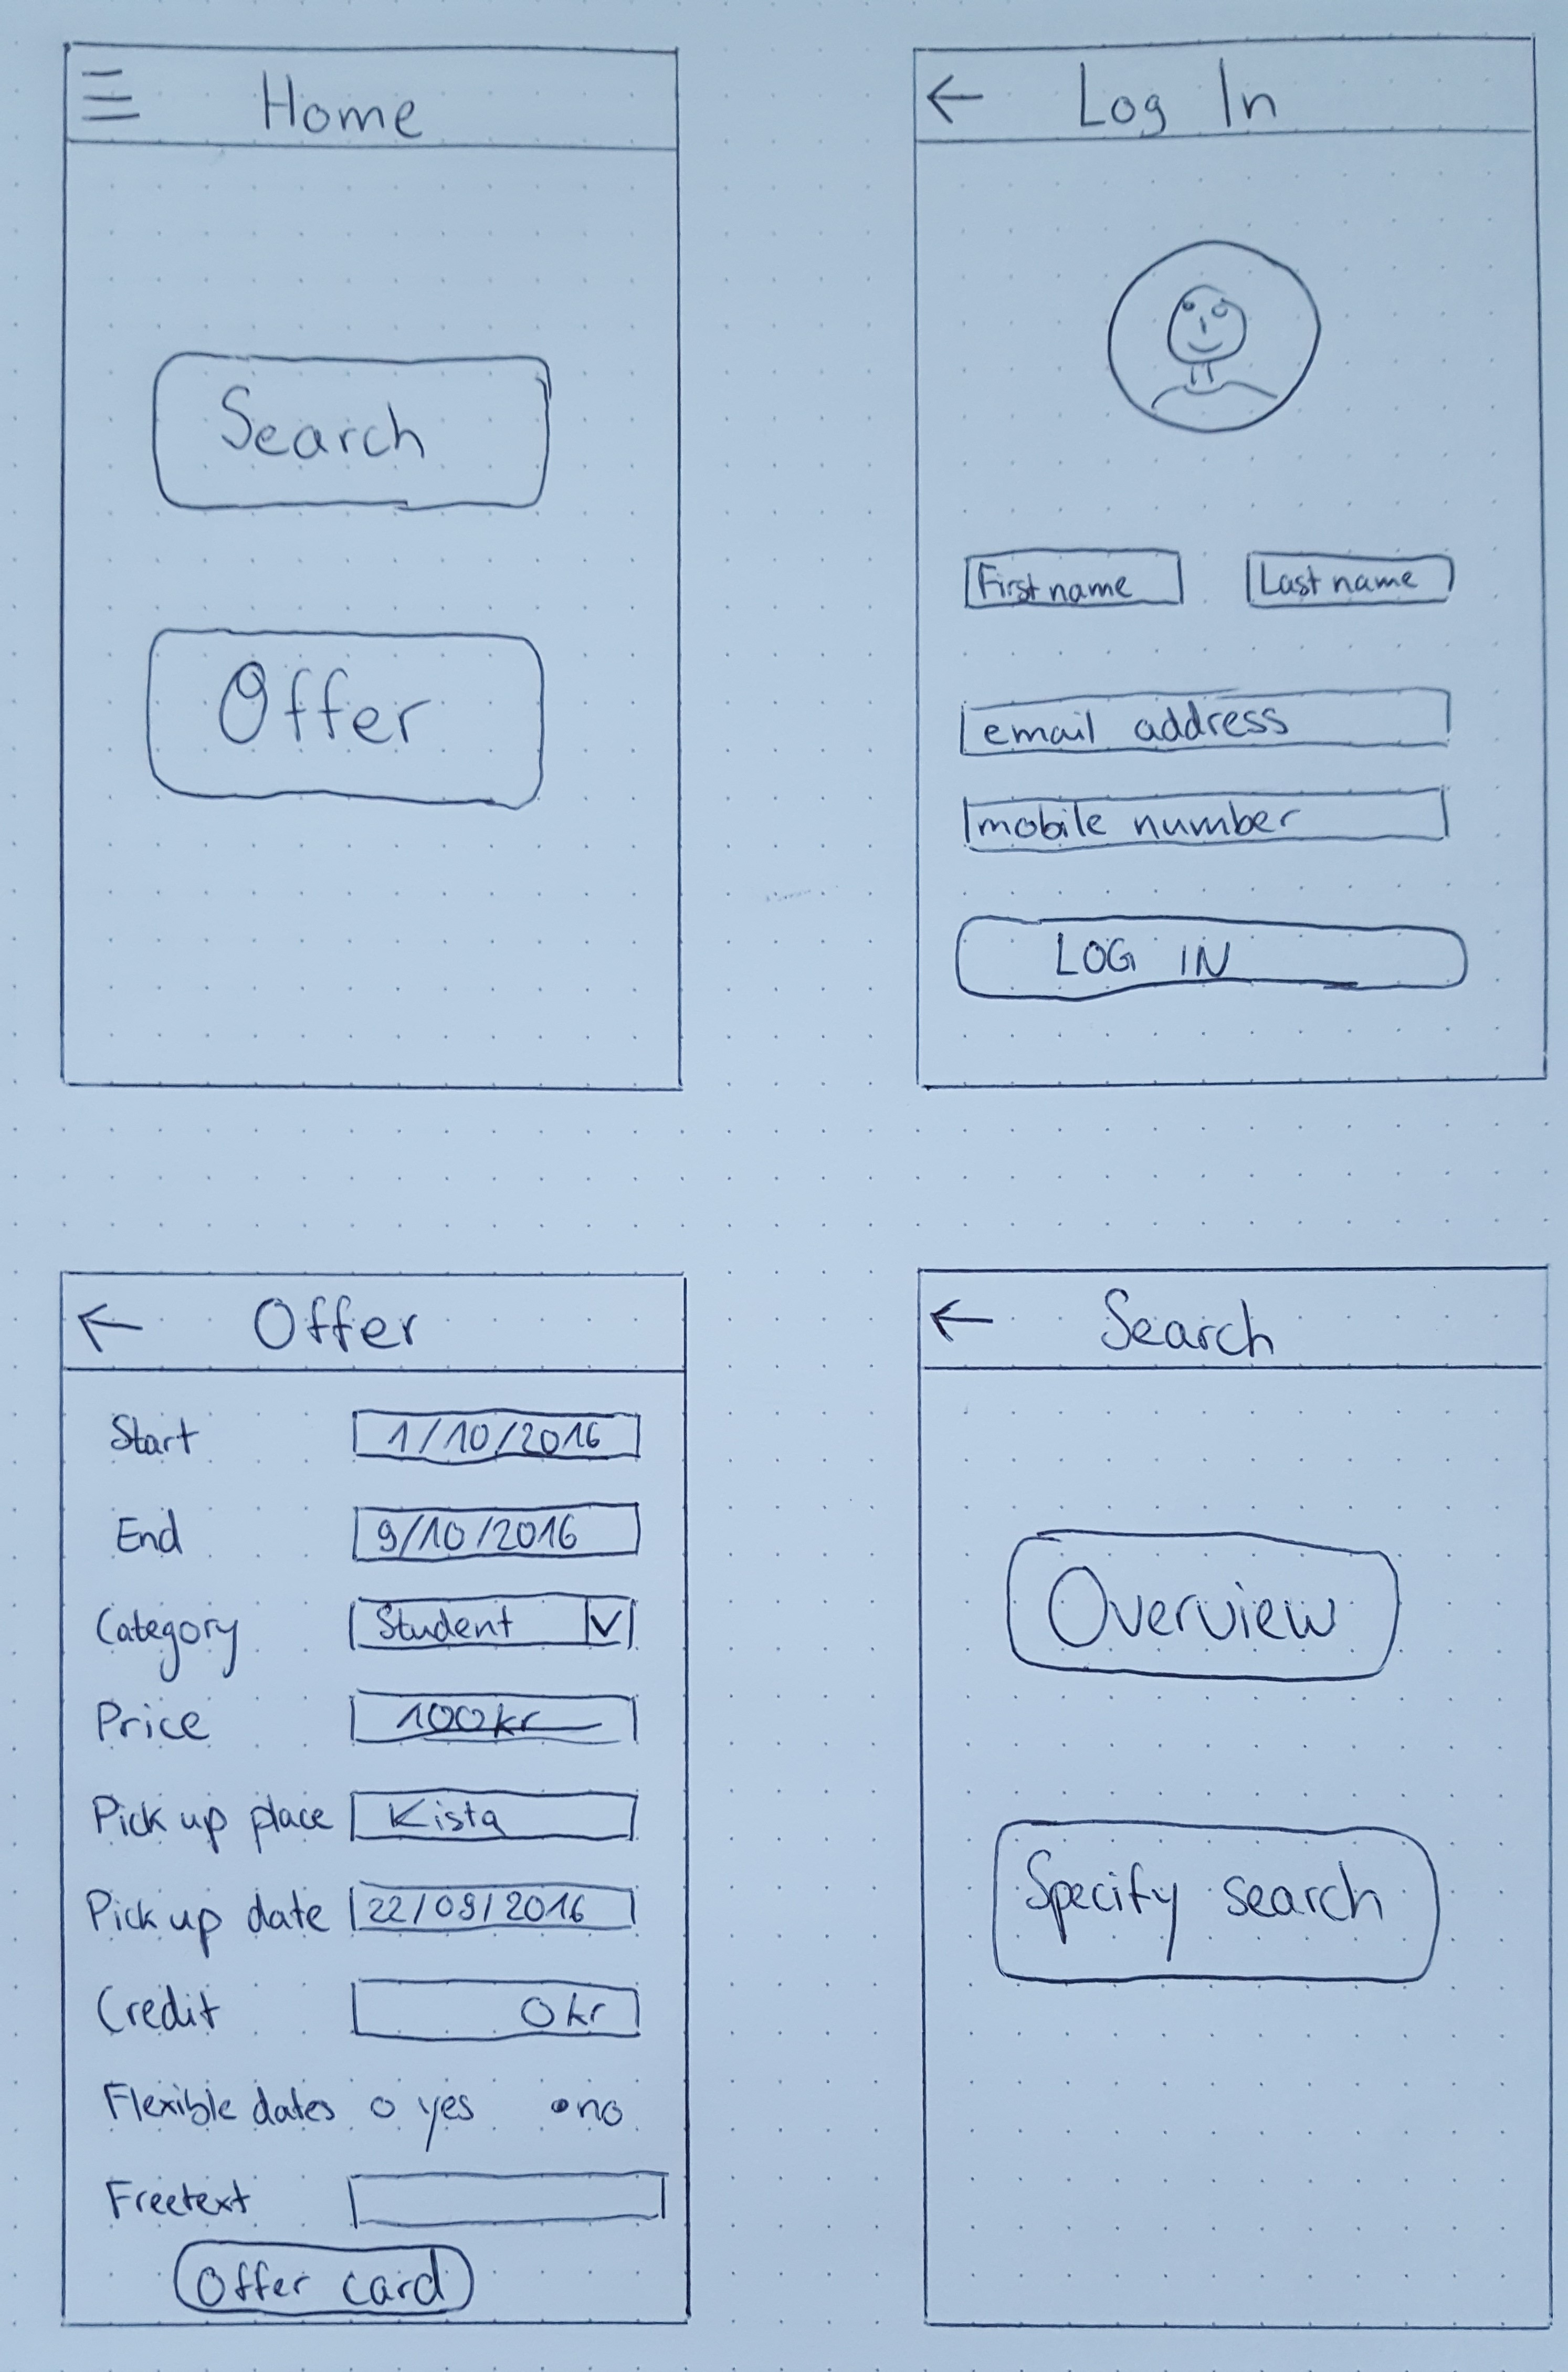
\includegraphics[width=\textwidth]{jpg/paper-prototype-1.jpg}
	\caption{Paper prototype figures}
	\label{figure:paper-prototype-1}
\end{figure}

\begin{figure}
	\centering
	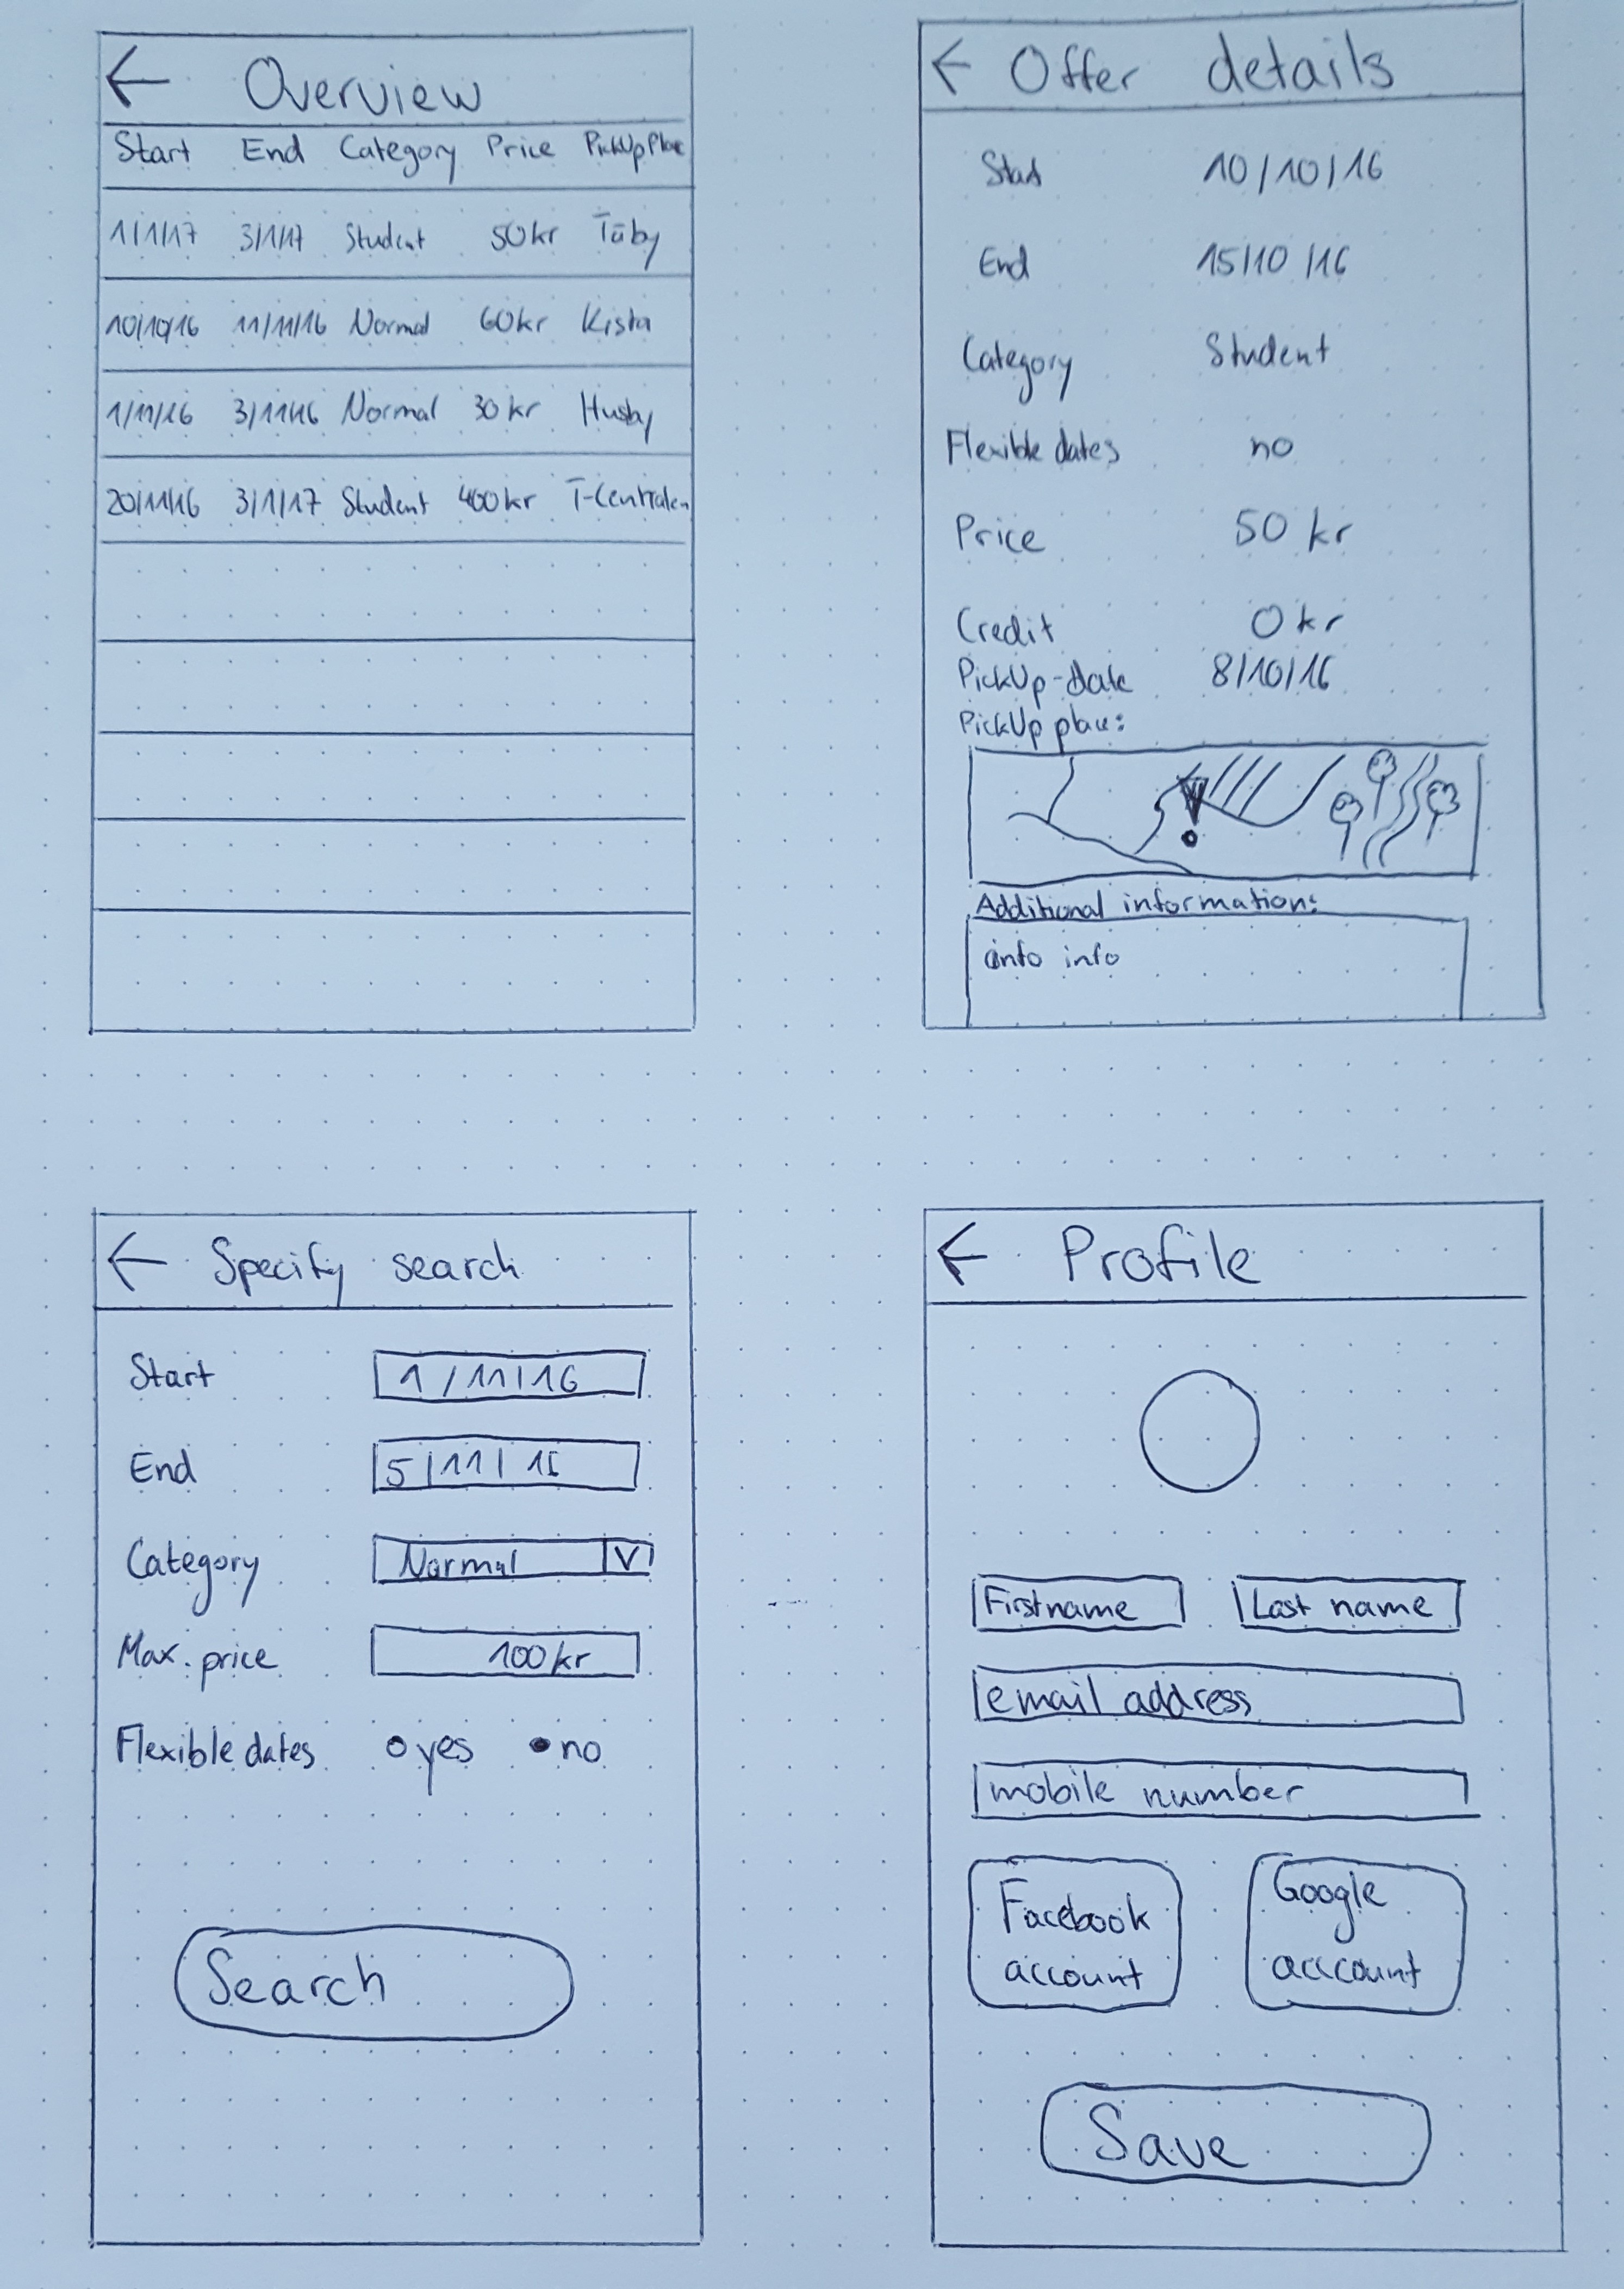
\includegraphics[width=\textwidth]{jpg/paper-prototype-2.jpg}
	\caption{Paper prototype}
	\label{figure:paper-prototype-2}
\end{figure}

\chapter{Site map and clickstream figures}
\newpage

\begin{figure}
	\centering
	\includegraphics[page=9,width=\textwidth]{pdf/balsamiq.pdf}
	\caption{Site map}
	\label{figure:site-map}
\end{figure}

\begin{figure}
	\centering
	\includegraphics[page=10,width=\textwidth]{pdf/balsamiq.pdf}
	\caption{Clickstream}
	\label{figure:clickstream}
\end{figure}

\chapter{WebApp prototype figures}
\label{webapp-prototype-appendix}
\newpage

\begin{figure}
	\centering
	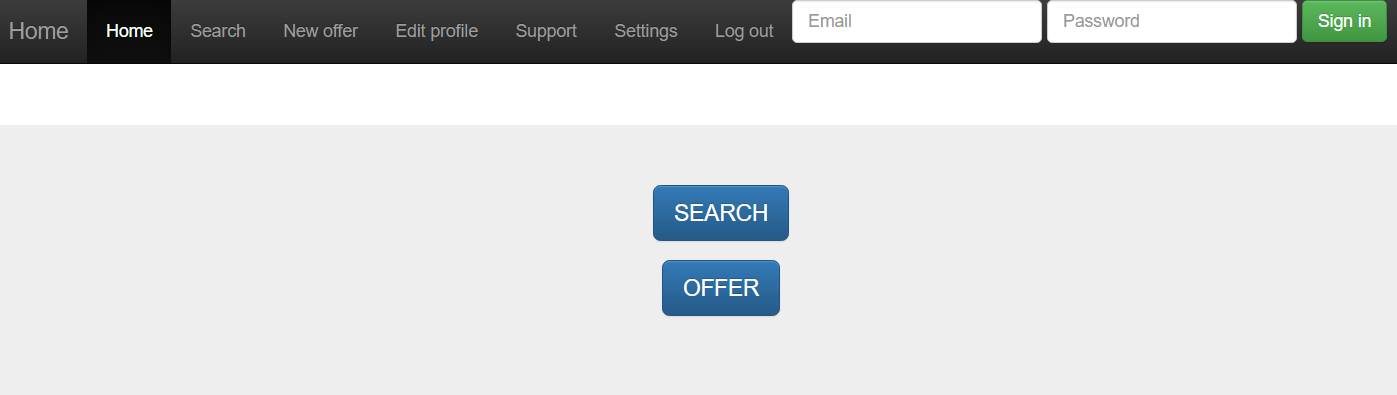
\includegraphics[width=\textwidth]{png/webapp-start.png}
	\caption{Start page}
	\label{figure:start-page}
\end{figure}

\begin{figure}
	\centering
	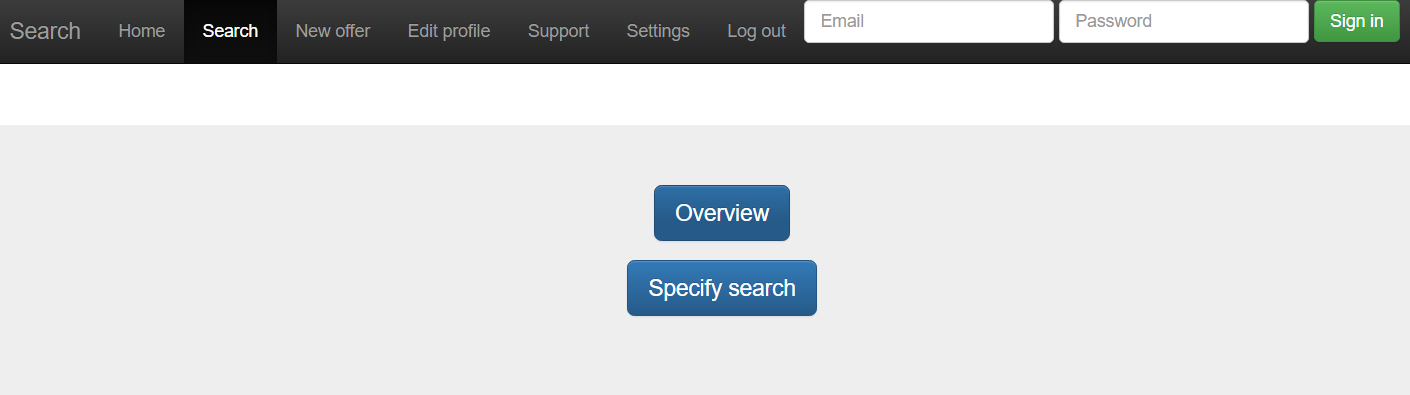
\includegraphics[width=\textwidth]{png/webapp-search.png}
	\caption{Search page}
	\label{figure:search-page}
\end{figure}

\begin{figure}
	\centering
	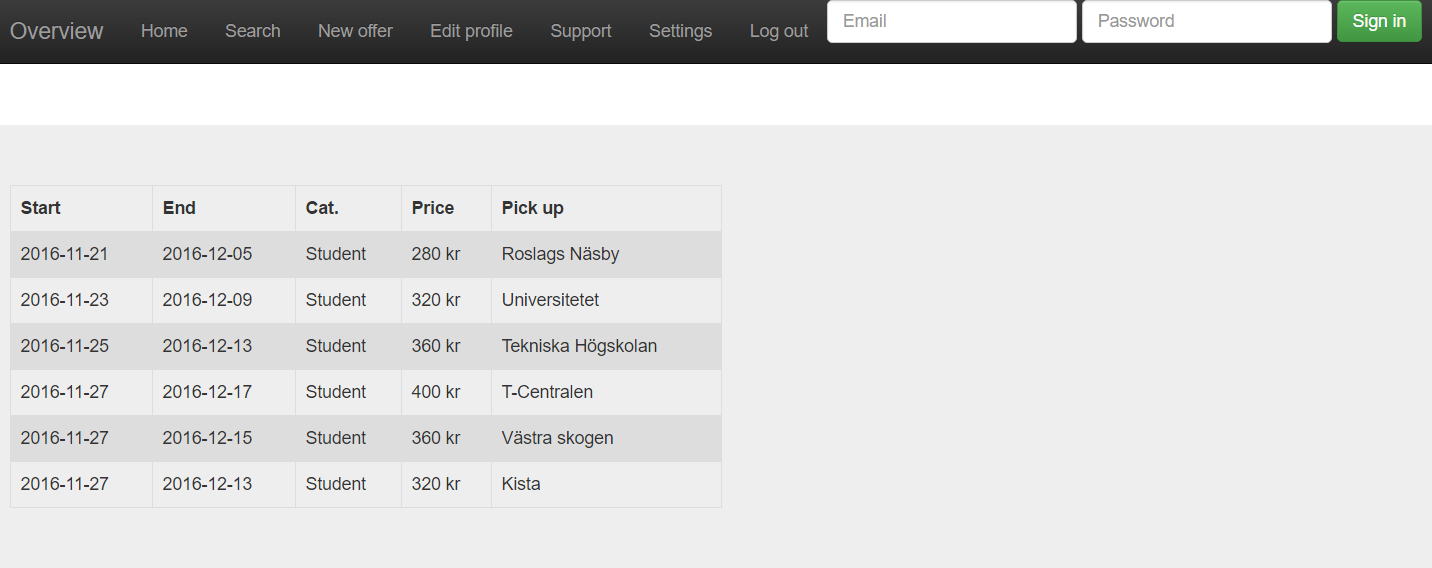
\includegraphics[width=\textwidth]{png/webapp-overview.png}
	\caption{Overview page}
	\label{figure:overview-page}
\end{figure}

\begin{figure}
	\centering
	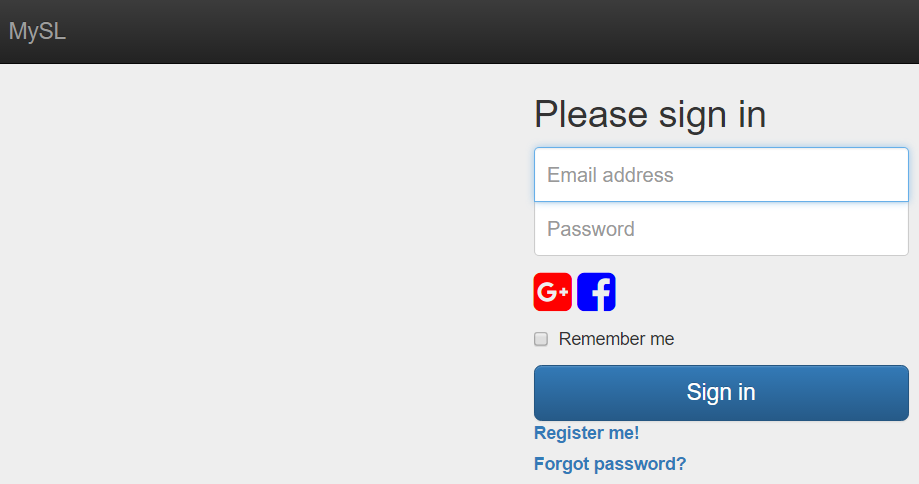
\includegraphics[width=\textwidth]{png/webapp-login.png}
	\caption{Login page}
	\label{figure:login-page}
\end{figure}

\begin{figure}
	\centering
	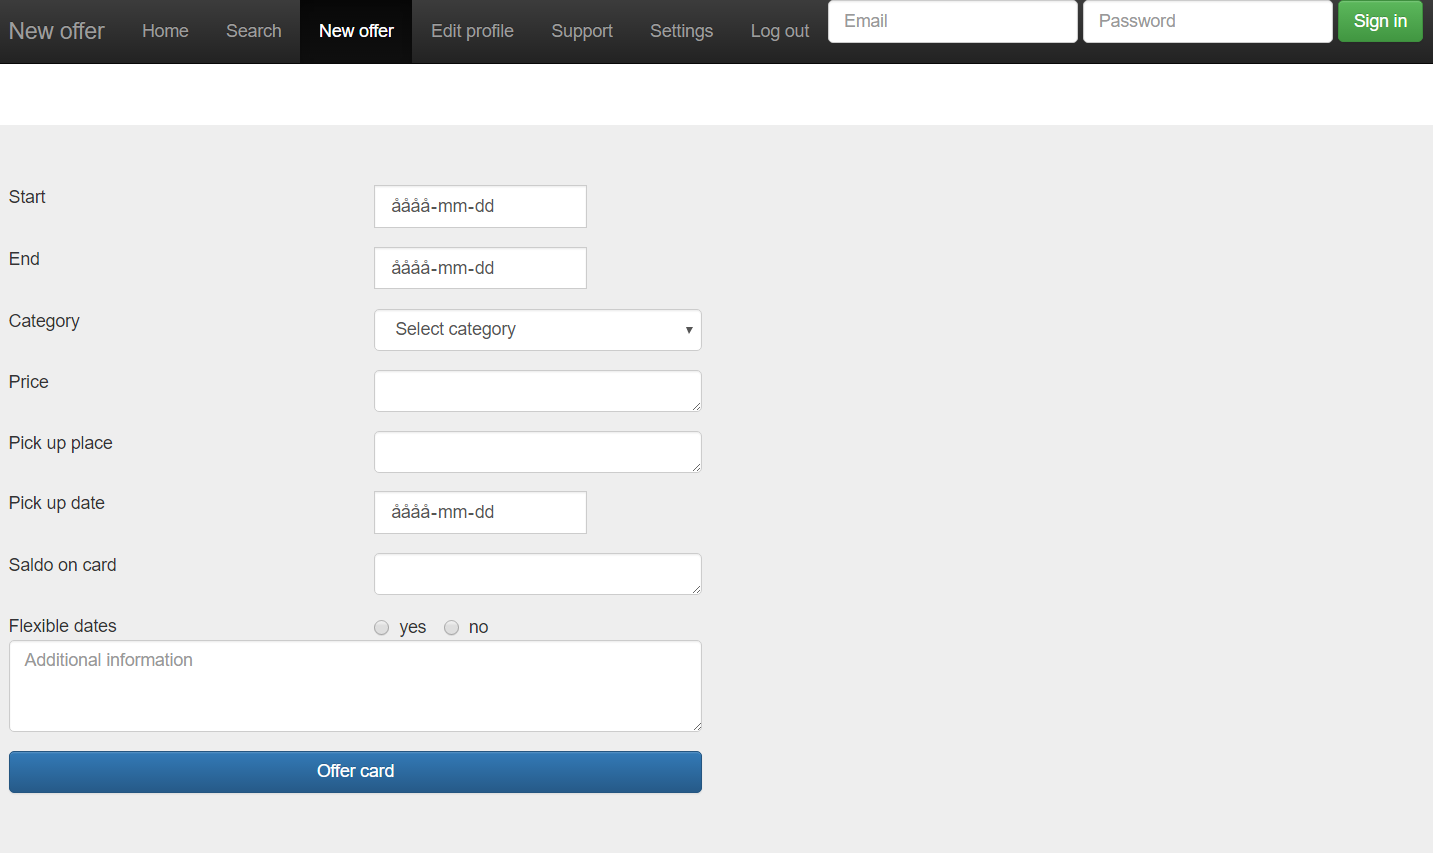
\includegraphics[width=\textwidth]{png/webapp-newoffer.png}
	\caption{New offer page}
	\label{figure:new-offer-page}
\end{figure}

\begin{figure}
	\centering
	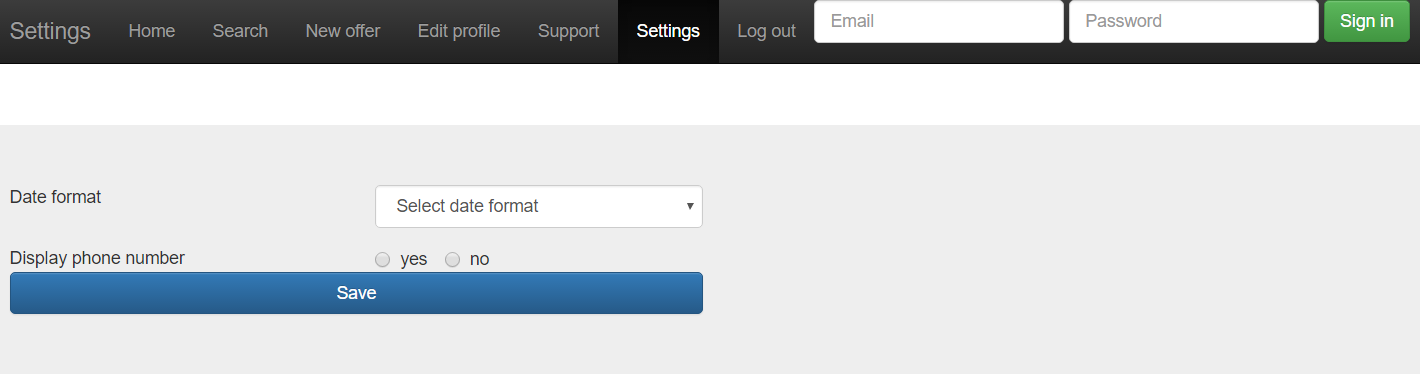
\includegraphics[width=\textwidth]{png/webapp-settings.png}
	\caption{Settings page}
	\label{figure:settings-page}
\end{figure}

\chapter{Android prototype figures}
\label{appendix:android-prototype-figures}
\newpage

\begin{figure}
	\centering
	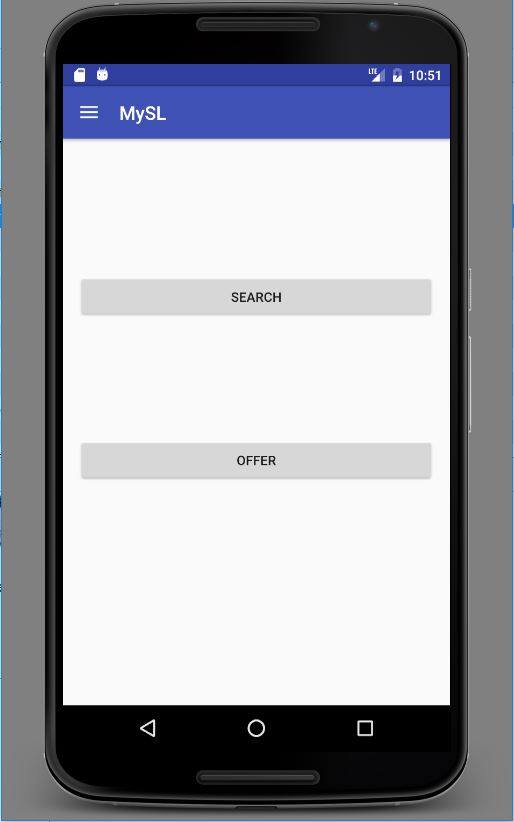
\includegraphics[width=0.4\textwidth]{jpg/android-start.jpg}
	\caption{Start view}
	\label{figure:start-view}
\end{figure}

\begin{figure}
	\centering
	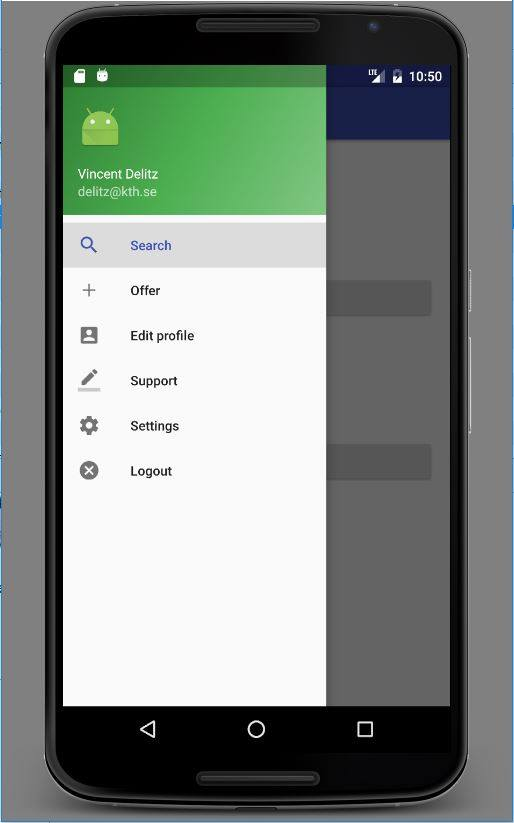
\includegraphics[width=0.4\textwidth]{jpg/android-navigation-drawer.jpg}
	\caption{Navigation drawer in start view}
	\label{figure:navigation-drawer-in-start-view}
\end{figure}

\begin{figure}
	\centering
	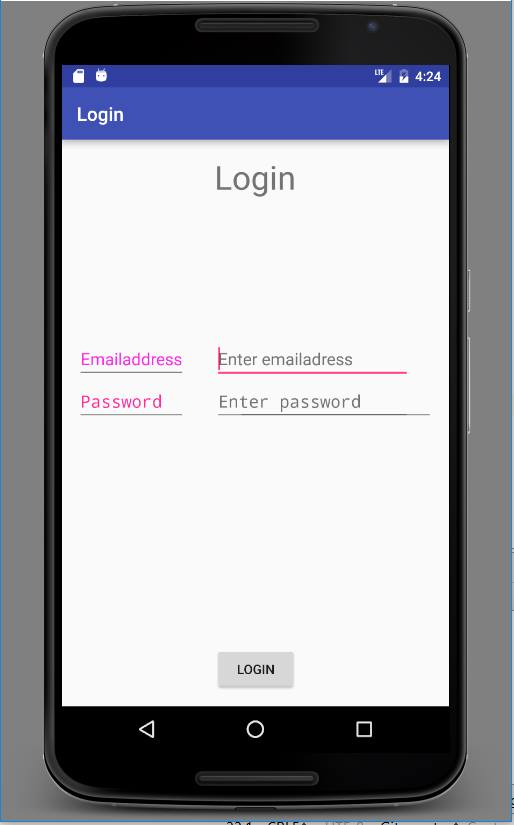
\includegraphics[width=0.4\textwidth]{png/android-login.png}
	\caption{Login view}
	\label{figure:navigation-drawer-in-start-view}
\end{figure}

\begin{figure}
	\centering
	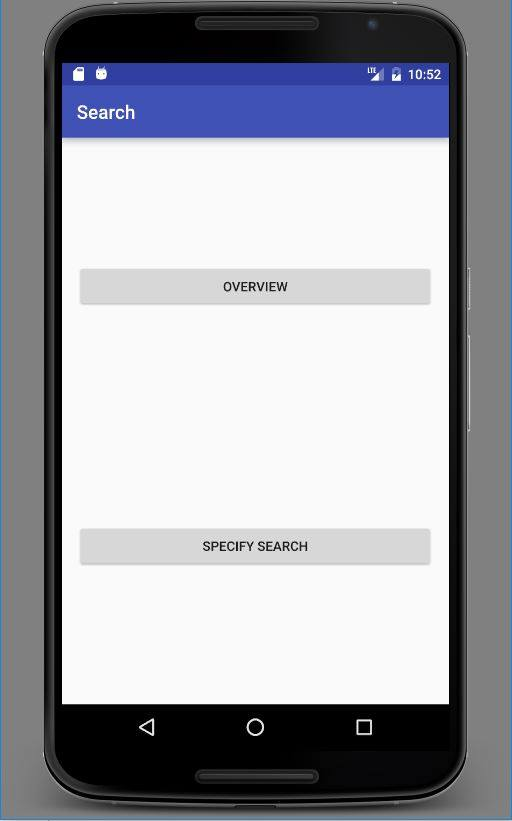
\includegraphics[width=0.4\textwidth]{jpg/android-search.jpg}
	\caption{Search view}
	\label{figure:search-view}
\end{figure}

\begin{figure}
	\centering
	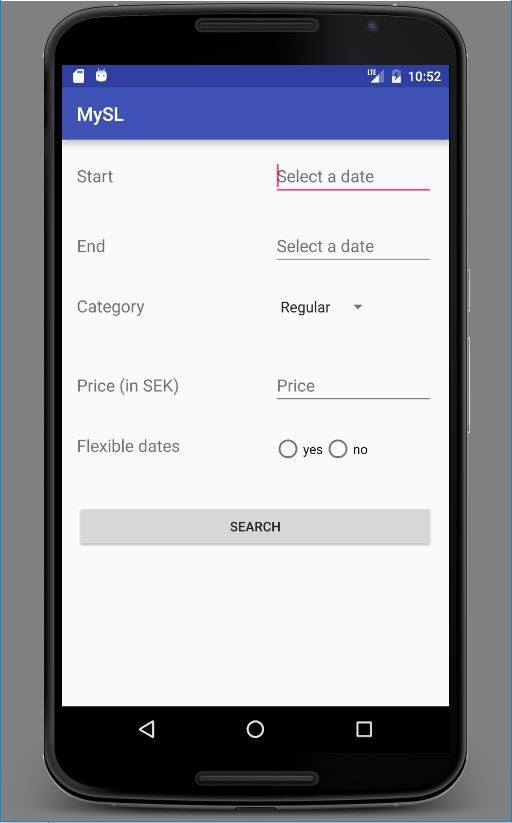
\includegraphics[width=0.4\textwidth]{jpg/android-specify-search.jpg}
	\caption{Specify search view}
	\label{figure:specify-search-view}
\end{figure}

\begin{figure}
	\centering
	\fcolorbox{black}{black}{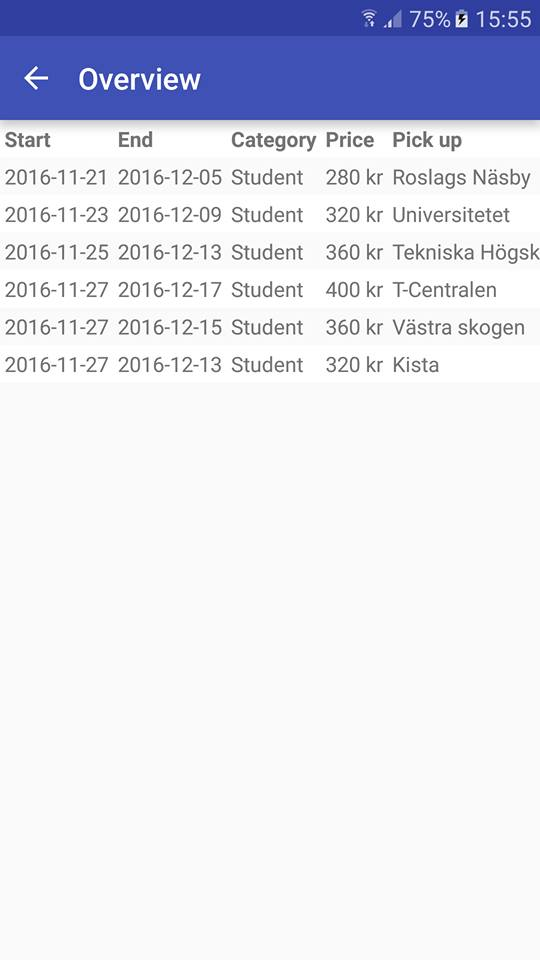
\includegraphics[width=0.4\textwidth]{png/android-overview.png}}
	\caption{Overview}
	\label{figure:overview}
\end{figure}

\begin{figure}
	\centering
	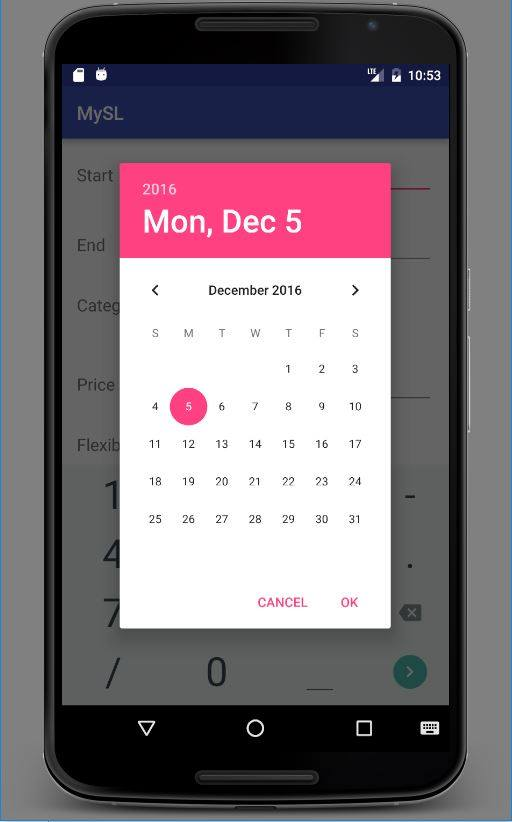
\includegraphics[width=0.4\textwidth]{jpg/android-calendar.jpg}
	\caption{Calendar view}
	\label{figure:calendar-view}
\end{figure}

\begin{figure}
	\centering
	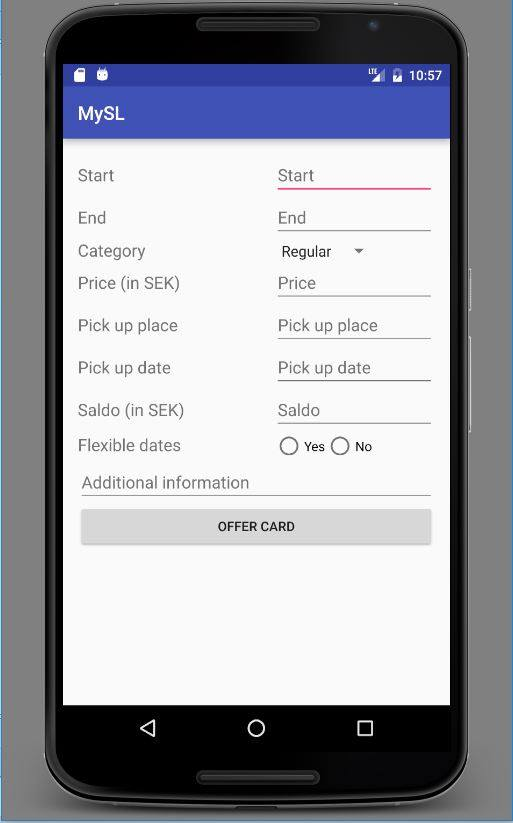
\includegraphics[width=0.4\textwidth]{jpg/android-offer.jpg}
	\caption{Offer view}
	\label{figure:offer-view}
\end{figure}

\chapter{App web service figures}
\label{appendix:app-web-service-figures}
\newpage

\begin{figure}
	\centering
	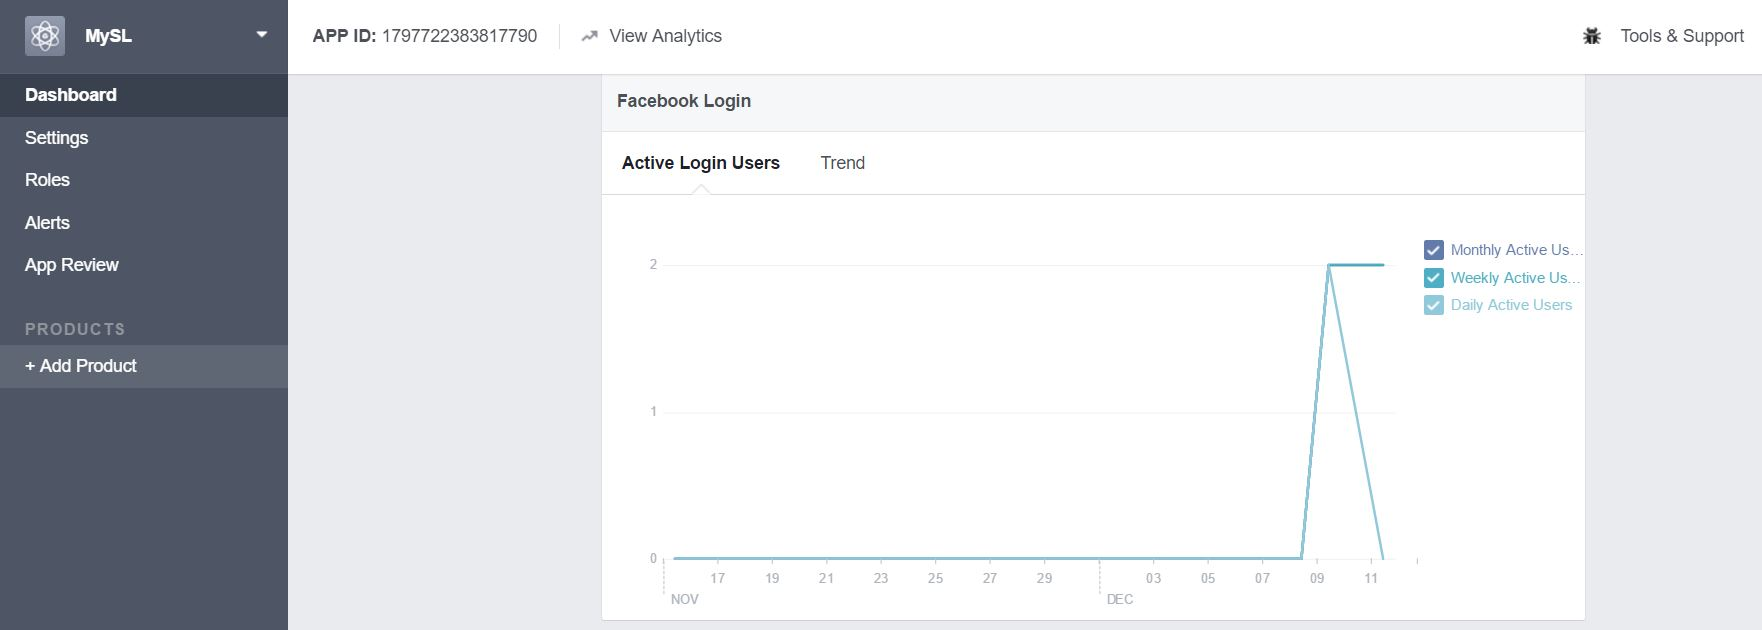
\includegraphics[width=1\textwidth]{jpg/facebook-developers.jpg}
	\caption{Facebook developers dashboard website}
	\label{figure:start-view}
\end{figure}

\begin{figure}
	\centering
	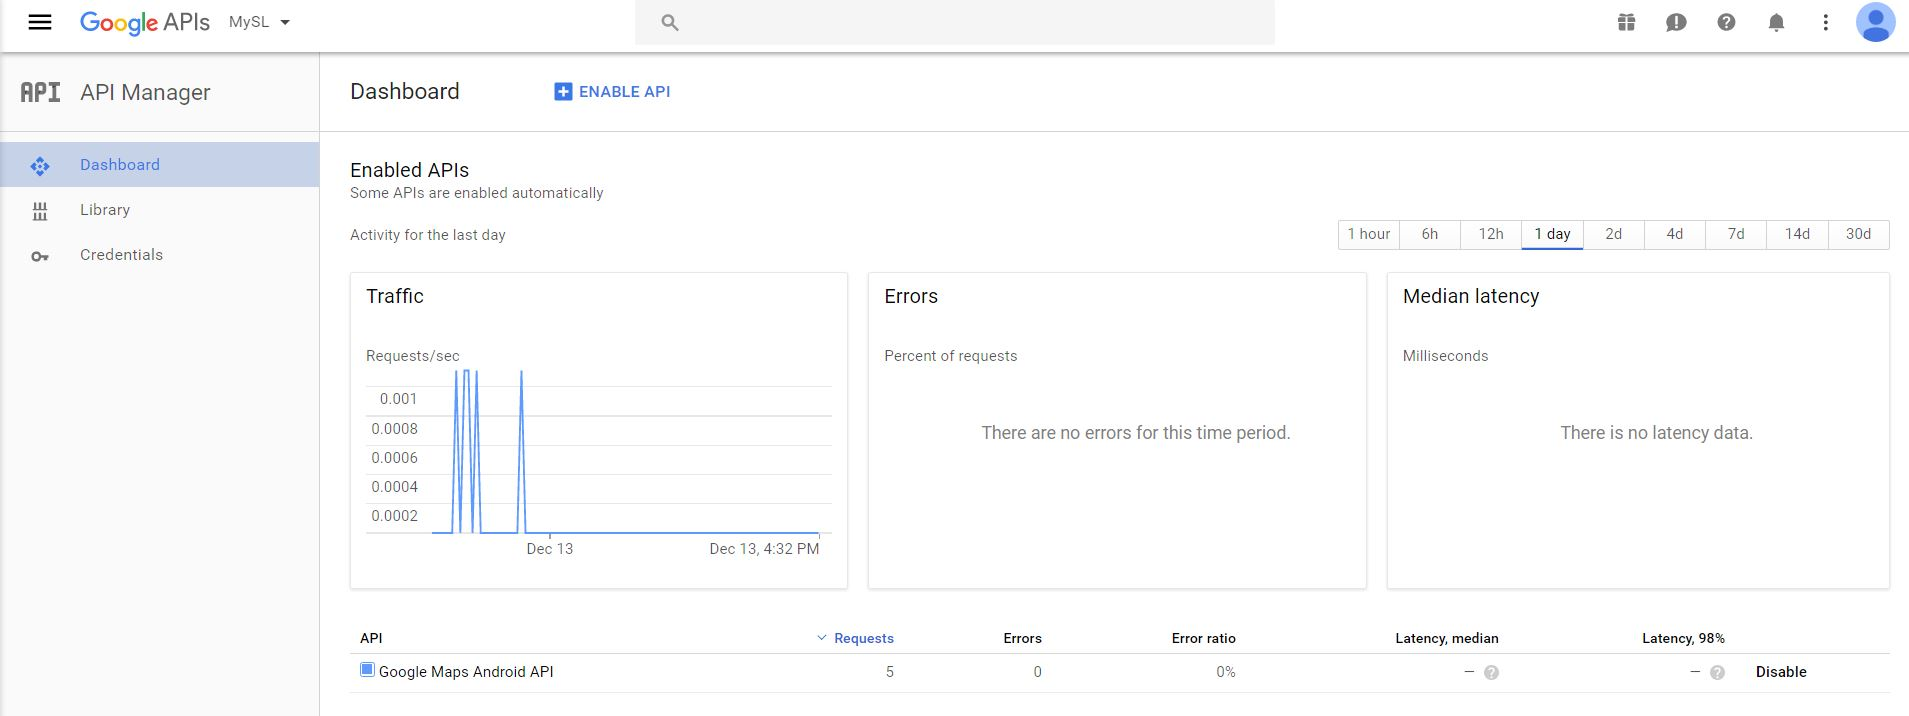
\includegraphics[width=1\textwidth]{jpg/google-developers.jpg}
	\caption{Google developers dashboard website}
	\label{figure:navigation-drawer-in-start-view}
\end{figure}

\begin{figure}
	\centering
	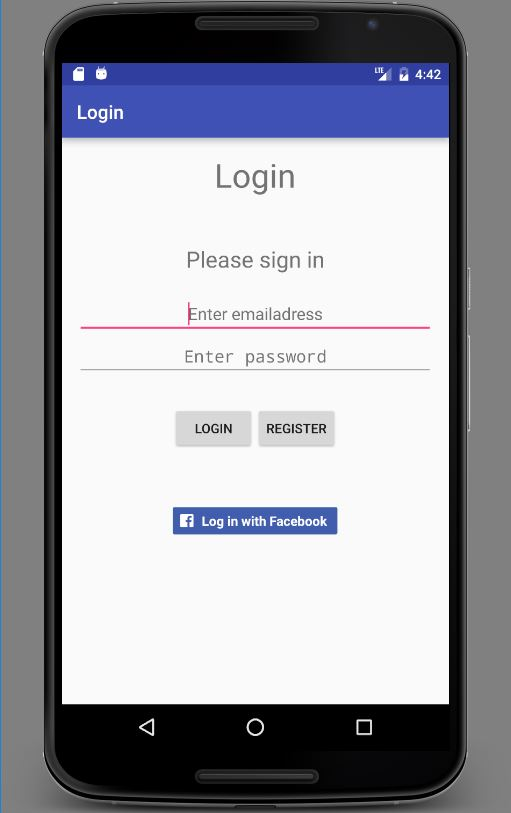
\includegraphics[width=0.4\textwidth]{jpg/facebook1.jpg}
	\caption{Login view with Facebook login button}
	\label{figure:navigation-drawer-in-start-view}
\end{figure}

\begin{figure}
	\centering
	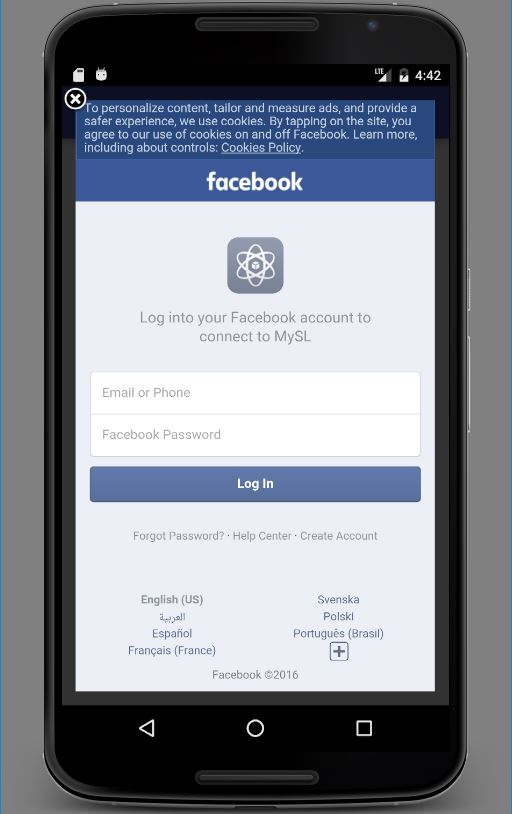
\includegraphics[width=0.4\textwidth]{jpg/facebook2.jpg}
	\caption{Integrated facebook login view}
	\label{figure:search-view}
\end{figure}

\begin{figure}
	\centering
	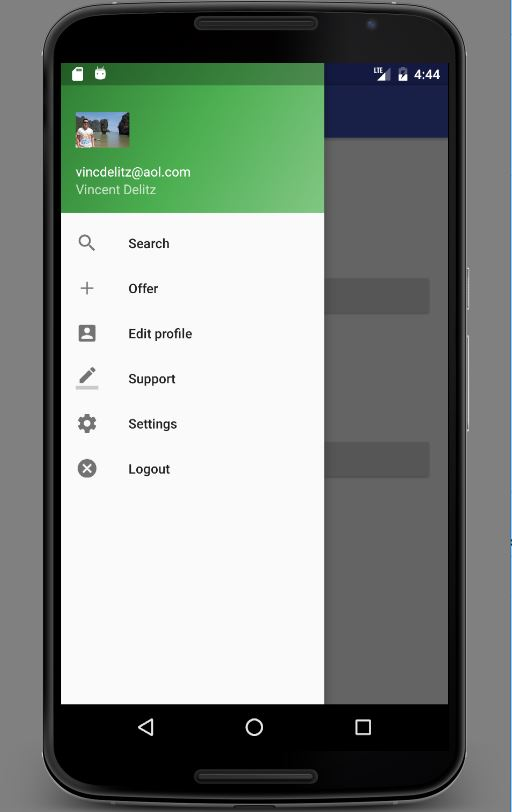
\includegraphics[width=0.4\textwidth]{jpg/facebook3.jpg}
	\caption{Pulled Facebook data and profile picture in the navigation drawer}
	\label{figure:specify-search-view}
\end{figure}

\begin{figure}
	\centering
	\fcolorbox{black}{black}{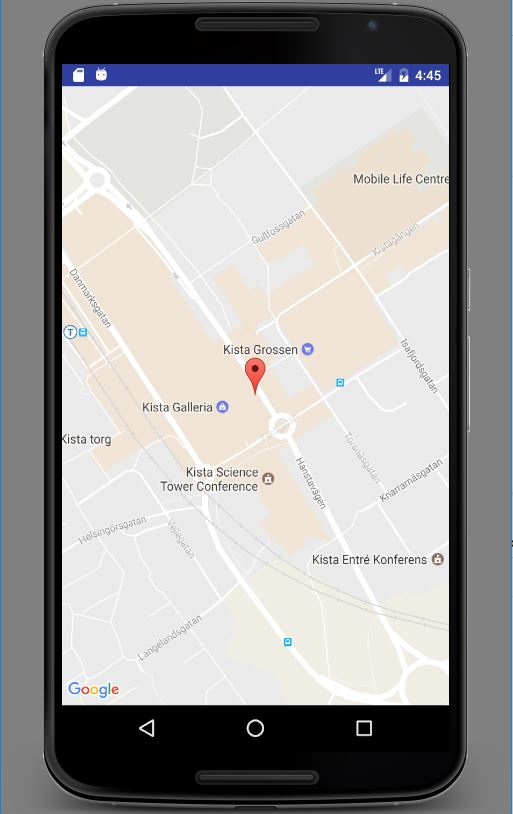
\includegraphics[width=0.4\textwidth]{jpg/google.jpg}}
	\caption{Integrated Google Maps for the pick-up place}
	\label{figure:overview}
\end{figure}

\chapter{Opposition report}
\label{appendix:opposition-report}
\newpage

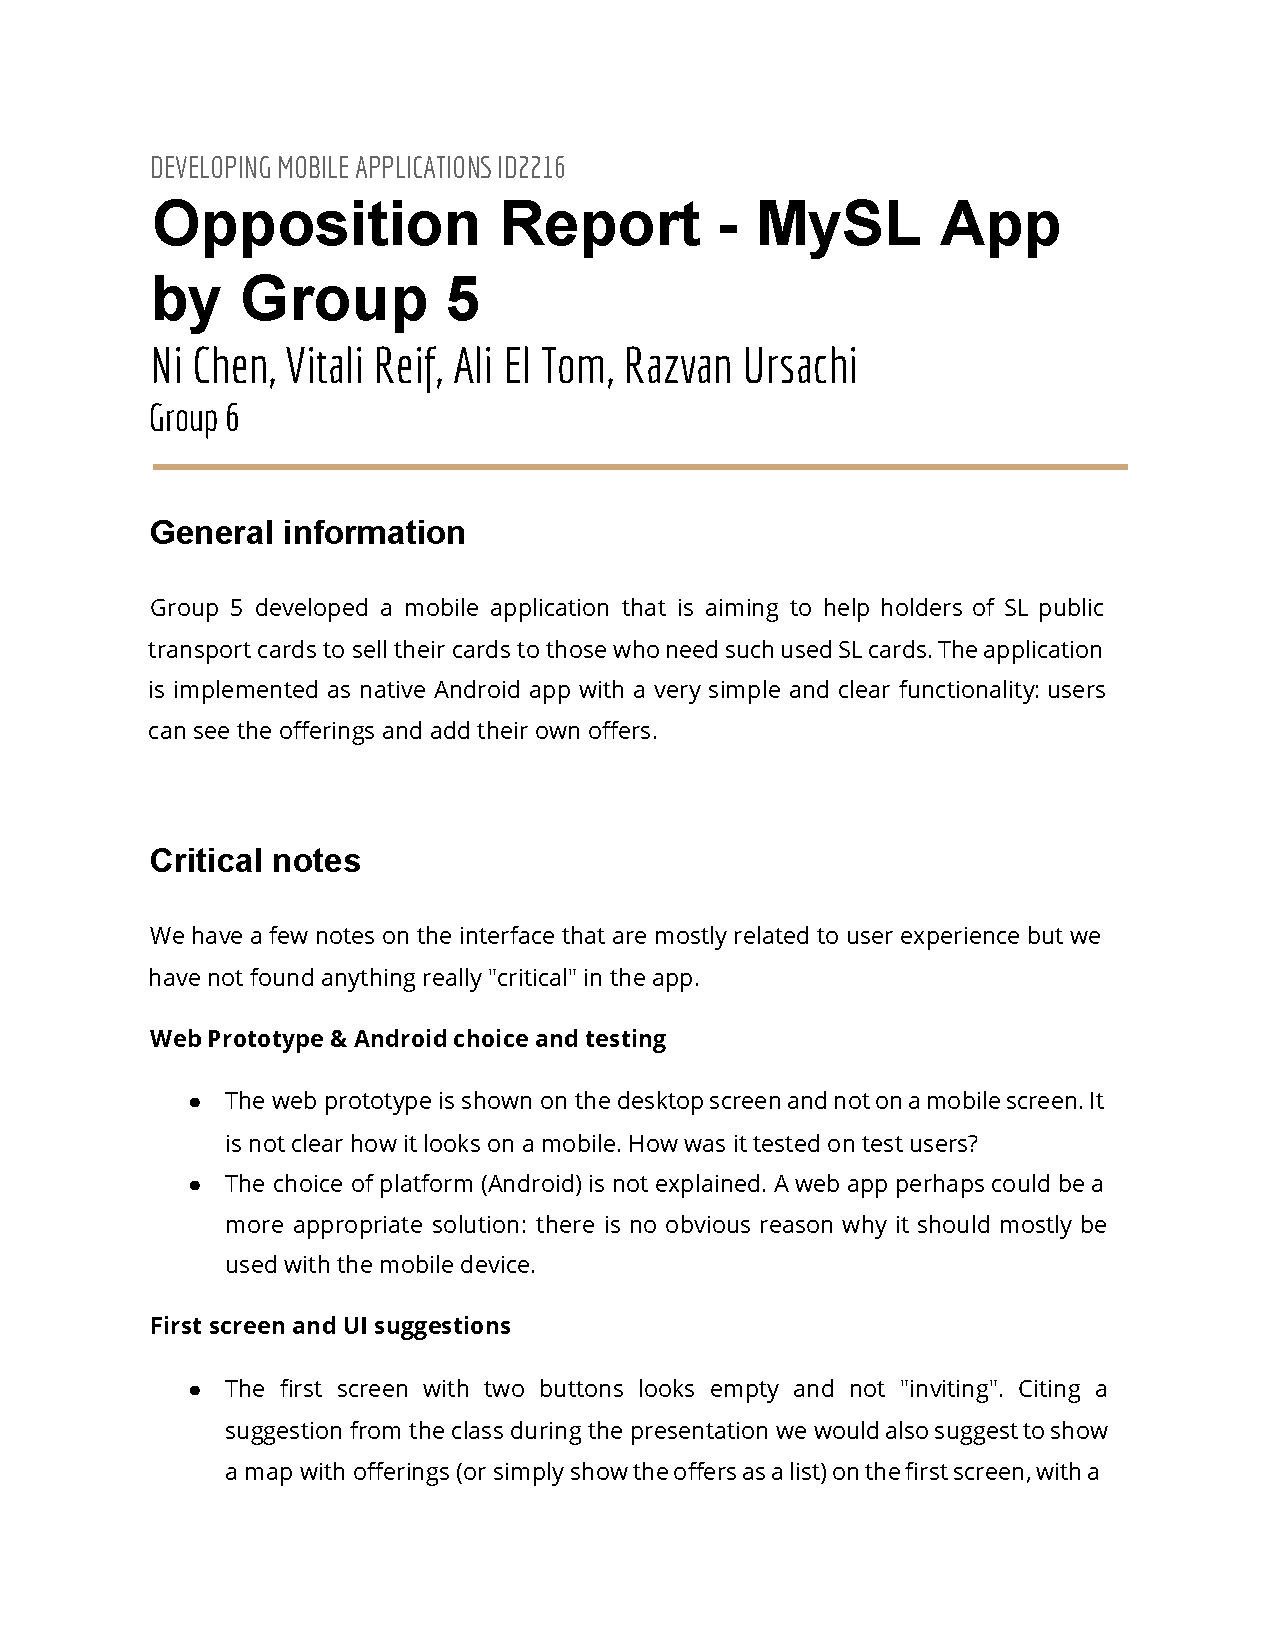
\includepdf[pages={-}]{pdf/Group5_project_review}

\end{appendices}

\begin{thebibliography}{9}

\bibitem{sl}
  SL General Sales and Travel Terms and Conditions,\\
  \url{https://sl.se/contentassets/36a0862a7c6a4c8ba0bf0da30e301043/general_terms_and_conditions_13october2016.pdf},\\
  13 October 2016.

\end{thebibliography}

\end{document}
